\documentclass[12pt,letterpaper]{article}

% ---------- Encoding, fonts, layout ----------
\usepackage[T1]{fontenc}
\usepackage[utf8]{inputenc}

  \usepackage{newtxtext, newtxmath}

\usepackage{geometry}
\geometry{margin=1in}

\usepackage{microtype}
\usepackage{setspace}
\setstretch{1.15}
\setlength{\parskip}{6pt plus 2pt minus 1pt}
\setlength{\parindent}{0pt}
\setlength{\emergencystretch}{3em}

\usepackage{tabularx}
\newcolumntype{Y}{>{\raggedright\arraybackslash}X}

% ---------- Graphics & tables ----------
\usepackage{graphicx}
\usepackage{booktabs}
\usepackage{longtable}
\usepackage{array}
\usepackage{float} % <-- enables [H] float placement
\IfFileExists{footnote.sty}{\usepackage{footnote}\makesavenoteenv{longtable}}{}

% 
% ---------- Links ----------
\usepackage{xcolor}
\definecolor{linkblue}{rgb}{0.0,0.2,0.6}
\usepackage{hyperref}
\hypersetup{
  colorlinks=true,
  linkcolor=linkblue,
  citecolor=linkblue,
  urlcolor=linkblue,
  breaklinks=true,
  pdftitle={},
  pdfauthor={}
}
\urlstyle{same}

% ---------- Header / footer ----------
\usepackage{fancyhdr}
\pagestyle{fancy}
\fancyhf{}

% Use shorttitle from YAML; fall back to full title if not provided
\newcommand{\ShortTitleText}{Anchor Method Evaluation}

% Default (all pages except the first): short title on the left, page number right
\lhead{\textsf{\ShortTitleText}}
\rhead{\textsf{\thepage}}
\setlength{\headheight}{15pt}
\renewcommand{\headrulewidth}{0.4pt}  % horizontal rule ON for subsequent pages

% First-page style: NO header rule, NO page number
\fancypagestyle{firstpage}{
  \fancyhf{}                 % clear header/footer
  \renewcommand{\headrulewidth}{0pt} % remove the line on first page
}

% ---------- Section titles (valid separation lengths) ----------
% ---------- Section titles (unnumbered) ----------
\setcounter{secnumdepth}{0}  % do not number sections at all

\usepackage[compact,sf,bf]{titlesec}
\titleformat{\section}[block]{\Large\bfseries\sffamily}{}{0.6em}{}        % no \thesection
\titleformat{\subsection}[block]{\normalsize\bfseries\sffamily}{}{0.5em}{} % no \thesubsection
\titleformat{\subsubsection}[block]{\normalsize\bfseries\sffamily}{}{0.5em}{}

\titlespacing{\section}{0pt}{*2}{*0.6}
\titlespacing{\subsection}{0pt}{*1.2}{*0.4}
\titlespacing{\subsubsection}{0pt}{*1.0}{*0.3}


% ---------- Captions ----------
\usepackage{caption}
\DeclareCaptionStyle{italic}[justification=raggedright,singlelinecheck=false]{labelfont={bf},textfont={it},labelsep=colon}
\captionsetup[figure]{style=italic,format=hang}
\captionsetup[table]{style=italic,format=hang}

% ---------- BibLaTeX (enabled only if bibliography is provided) ----------
\usepackage[style=authoryear-comp,backend=biber,natbib=true,maxnames=3]{biblatex}
\addbibresource{../anchor_memo.bib}

% ---------- BibLaTeX (enabled only if bibliography is provided) ----------
% Configure BibLaTeX for American Fisheries Society (AFS) style
% \PassOptionsToPackage{
%   backend=biber,     % Core processing engine
%   style=authoryear,  % Author-Year format
%   maxcitenames=2,    % Use 'et al.' for more than 2 authors in text
%   maxbibnames=99,    % List all authors in the bibliography
%   uniquename=false,  % Turn off initials for conflicting last names
%   uniquelist=false
% }{biblatex}
% 
% % AFS Specific Tweaks:
% \AtBeginDocument{
%   % Remove the comma between Author and Year in text citations: e.g., (Kinzer 2026)
%   \DeclareDelimFormat{nameyeardelim}{\addspace} 
%   
%   % Separate multiple entries with semicolons: e.g., (Kinzer 2026; Briggs 2025)
%   \DeclareDelimFormat{multicitedelim}{\addsemicolon\space}
% }


% ---------- Optional watermark ----------
\usepackage{draftwatermark}
\SetWatermarkText{DRAFT}
\SetWatermarkScale{0.9}
\SetWatermarkColor[gray]{0.9}

% ---------- tcolorbox (memo header + callouts) ----------
\usepackage[most]{tcolorbox}
\tcbset{boxrule=0.5pt,arc=2mm,left=6pt,right=6pt,top=6pt,bottom=6pt}

% Executive Summary / Recommendations environments (optional)
\newenvironment{execsum}{%
  \begin{tcolorbox}[colback=blue!3,colframe=blue!50!black,title=\textbf{Executive Summary}]
}{\end{tcolorbox}}

\newenvironment{recs}{%
  \begin{tcolorbox}[colback=green!3,colframe=green!40!black,title=\textbf{Recommendations}]
}{\end{tcolorbox}}

% ---------- Branding (logos), only if branding: yes ----------
\usepackage[absolute,overlay]{textpos}
\setlength{\TPHorizModule}{1cm}
\setlength{\TPVertModule}{1cm}

% ---------- Memo header box ----------
\newcommand{\MemoHeader}{%
      \vspace*{2cm}% push content down if branding block is present
    \begin{tcolorbox}[colback=gray!5,colframe=gray!45,coltitle=black, center title, title=\textbf{Technical Memorandum}]
    \begin{tabularx}{\textwidth}{@{}p{2.2cm} Y@{}}
      \textbf{To} &
        \begin{minipage}[t]{\linewidth}\raggedright
          \setlength{\parindent}{0pt}%
          Jason Vogel, DFRM Research Division Director\\ William Young, DFRM Hatchery Evaluations Coordinator\\ Becky Johnson, DFRM Production Division Director
        \end{minipage}
      \\
      \textbf{From} &
        \begin{minipage}[t]{\linewidth}\raggedright
          \setlength{\parindent}{0pt}%
          Ryan N. Kinzer, DFRM Fisheries Data Analysis Coordinator
        \end{minipage}
      \\
            \textbf{CC} &
        \begin{minipage}[t]{\linewidth}\raggedright
          \setlength{\parindent}{0pt}%
          Brian Simmons, DFRM Research RM\&E Lead\\ Kyle Bratcher, ODFW Northeast Oregon Fish Manager
        \end{minipage}
      \\
            \textbf{Date}    & 28 August, 2026 \\
      \textbf{Subject} & Review of ODFW's Proposed North East Oregon Weir Management Framework \\
      
      
    \end{tabularx}
  \end{tcolorbox}
}


% ---------- Title metadata ----------
  \title{}

  \author{%
          \textbf{}\\
          }

\date{28 August, 2026}

% --- Pandoc tight list shim (prevents \tightlist error) ---
\providecommand{\tightlist}{%
  \setlength{\itemsep}{0pt}\setlength{\parskip}{0pt}}

% -------------------- BODY --------------------
\begin{document}

% Branding logos (optional)
  \begin{textblock}{3}(1,1.1)
\includegraphics[height=2.0cm]{../../templates/NPT.png}\end{textblock}
   \begin{textblock}{14}(3.75,0.5)
      \begin{center}
        {\LARGE Nez Perce Tribe}\\[0.1em]
        {\bfseries\Large Department of Fisheries Resources Management}\\[0.1em]
        {\bfseries\footnotesize Administration \textbullet Enforcement \textbullet Habitat/Watershed \textbullet Harvest \textbullet Production \textbullet Research}\\[0.1em]
        {\bfseries\normalsize Research Division}\\[0.1em]
        {\footnotesize P.O. Box 365 \textbullet Lapwai, Idaho 83540}\\[0.1em]
        {\footnotesize Phone: (208) 843-7145 \textbullet Fax: (208) 843-7310}\\[0.1em]        
      \end{center}
    \end{textblock}
  \begin{textblock}{3}(19,1.1)
\includegraphics[height=2.0cm]{../../templates/DFRM.png}\end{textblock}

% (Small title for PDF metadata clarity)
{\large\bfseries\sffamily }\par\vspace{0.4em}

% Make the FIRST page clean: no line, no page number
\thispagestyle{firstpage}

% Memo header
\MemoHeader

% Optional Executive Summary / Recommendations if provided via variables


% Content injection hooks

\section{Background}\label{background}

The Lostine River spring Chinook (Oncorhynchus tshawytscha) hatchery program is an integrated supplementation program intended to rebuild and maintain the naturally spawning population while providing harvest opportunities and meeting Tribal and mitigation obligations. Management of returning adults requires balancing these objectives through decisions regarding harvest, broodstock collection, natural spawning, and hatchery-origin fish management \autocite{npt_hatchery_2011}.

Since implementation of the Lostine River Hatchery and Genetic Management Plan (HGMP; \textcite{npt_hatchery_2011}), management at the Lostine River weir has been guided by a stepped ``sliding scale'' developed cooperatively by the Oregon Department of Fish and Wildlife (ODFW), Nez Perce Tribe (NPT), and Confederated Tribes of the Umatilla Indian Reservation (CTUIR). The sliding scale recognizes that management priorities change with natural-origin abundance. At low abundance, management emphasizes demographic support and natural spawning abundance, while at higher abundance it progressively increases the contribution of natural-origin fish to broodstock and limits hatchery-origin spawning.

ODFW recently developed an alternative accounting framework referred to as the Anchor Method. The proposed method retains the existing harvest framework and biological objectives but replaces the stepped sliding-scale approach for allocating adults at the weir with a continuous relationship between natural-origin abundance, broodstock composition, and natural spawning needs.

The purpose of this memorandum is to evaluate the proposed Anchor Method relative to the existing sliding-scale framework. Specifically, this review:

\begin{enumerate}
\def\labelenumi{\arabic{enumi}.}
\tightlist
\item
  Describes the biological rationale and accounting structure of the Anchor Method.
\item
  Compares historical management outcomes under the Anchor Method and existing sliding scale.
\item
  Evaluates the sensitivity of Anchor Method outcomes across a range of natural-origin abundance, hatchery-origin abundance, and spawner-goal scenarios.
\end{enumerate}

The intent of this review is to identify how the Anchor Method changes management outcomes, evaluate its strengths and limitations, and determine whether it provides a more consistent and biologically defensible approach to Lostine River weir management.

\section{Current Weir Management Framework}\label{current-weir-management-framework}

Management of returning adults occurs through two complementary but distinct decision frameworks: (1) the harvest framework described in the Grande Ronde Fishery Management and Evaluation Plan (FMEP; \textcite{odfw_and_wdfw_fishery_2021}), and (2) the weir management framework described in the HGMP \autocite{npt_hatchery_2011}. These frameworks operate sequentially but address different management decisions.

The FMEP establishes allowable harvest impacts based on preseason and inseason estimates of natural-origin (NOR) abundance. Harvest is applied first, determining the number of NOR and hatchery-origin (HOR) adults expected to remain available for management at the weir. The sliding scale is then applied to those post-harvest adults to determine broodstock collection, natural spawning, HOR passage above the weir, and HOR removal. Thus, the harvest framework determines the number of adults available for weir management, while the sliding scale determines how those adults are allocated after fisheries have occurred.

This distinction is important when evaluating the Anchor Method because it proposes to replace only the weir accounting component of the existing framework. The FMEP harvest framework, treaty allocations, and underlying biological objectives are unchanged. Figure \ref{fig:current-framework} illustrates the sequence of management decisions and identifies the portion of the existing framework that would be replaced by the Anchor Method.

\begin{figure}[H]

{\centering 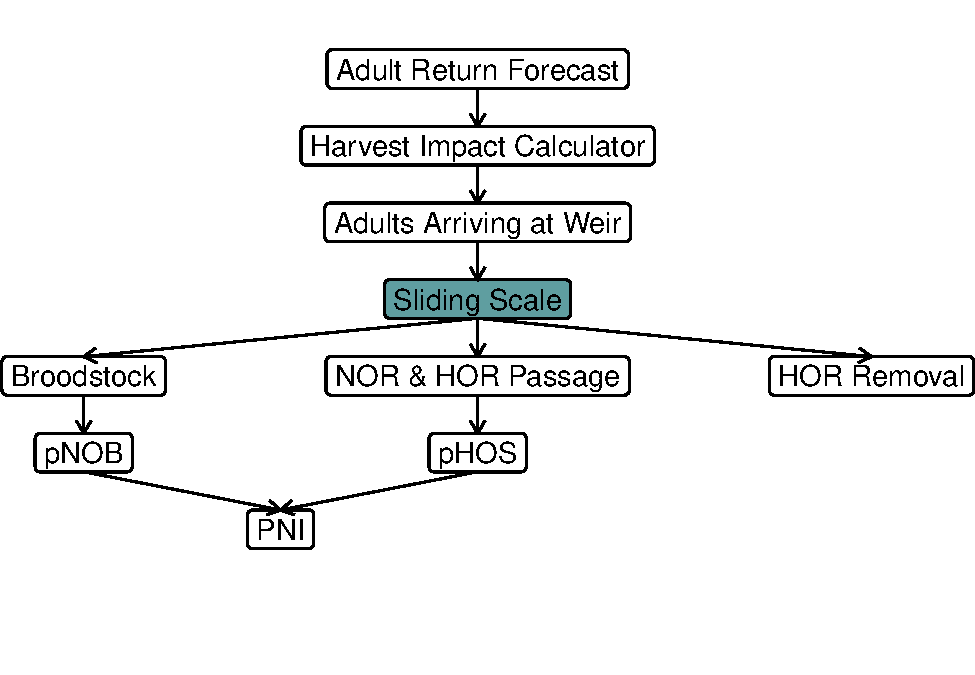
\includegraphics[width=1\linewidth]{anchor_method_evaluation_files/figure-latex/current-framework-1} 

}

\caption{Conceptual overview of the existing Lostine River management framework.}\label{fig:current-framework}
\end{figure}

\subsection{Harvest Impact Calculator}\label{harvest-impact-calculator}

Harvest is managed independently through the Grande Ronde FMEP \autocite{odfw_and_wdfw_fishery_2021}. Preseason forecasts of natural-origin abundance are combined with the Critical Threshold (CT) and Minimum Abundance Threshold (MAT) to determine allowable fishery impacts. Allowable harvest increases as natural-origin abundance increases while maintaining sufficient escapement to satisfy conservation objectives (Figure \ref{fig:fmep-harvest-impacts}).

Within the FMEP, preliminary harvest levels are first estimated using abundance-based harvest relationships. Those harvest levels are subsequently evaluated relative to broodstock requirements. If projected harvest would prevent broodstock goals from being achieved, harvest impacts are reduced until sufficient adults remain to satisfy broodstock needs. Consequently, broodstock protection places an upper limit on allowable harvest rather than harvest being an independent management objective.

Once fisheries have concluded, the remaining adults are managed at the weir according to the sliding scale.

\begin{figure}[H]

{\centering 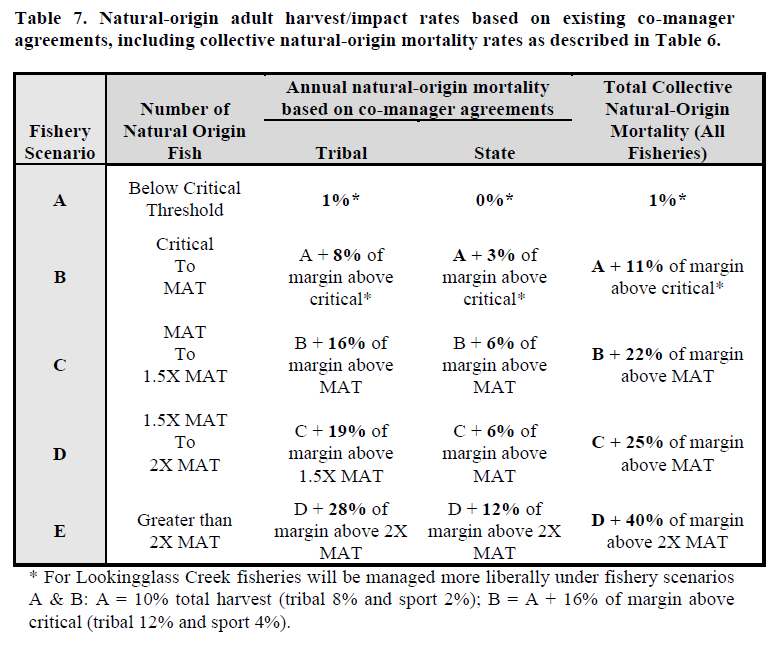
\includegraphics[width=1\linewidth]{./fmep_harvest_impacts} 

}

\caption{Copied from the 2012 Fisheries Management and Evaluation Plan for Spring Chinook in the Grande Ronde Subbasin.}\label{fig:fmep-harvest-impacts}
\end{figure}

\subsection{Existing Sliding Scale}\label{existing-sliding-scale}

The sliding scale was developed during implementation of the Lostine River integrated supplementation program to balance multiple management objectives that change as population abundance varies. Rather than applying a single management strategy across all return sizes, the sliding scale acknowledges that demographic and genetic risks differ between years of low and high abundance, and must be treated accordingly.

At low natural-origin abundance, demographic risk to population persistence was considered the greatest concern (Figure \ref{fig:lostine-sliding-scale}). Management therefore emphasized maximizing the total number of adults spawning naturally, even if this required allowing relatively large numbers of hatchery-origin fish upstream. Broodstock collection also relied more heavily on hatchery-origin fish because the relatively few natural-origin adults available were prioritized for natural spawning.

As natural-origin abundance increased, demographic risks diminished and management progressively shifted toward reducing genetic risks associated with hatchery supplementation. Greater numbers of natural-origin adults were incorporated into the broodstock, hatchery-origin fish passage above the weir was reduced, and hatchery-origin removals increased. This transition was implemented through a stepped relationship between natural-origin abundance and desired broodstock composition (Figure \ref{fig:lostine-sliding-scale}).

Although pNOB, pHOS, and PNI are now widely used to evaluate integrated and segregated hatchery programs, they were not explicitly managed under the sliding-scale approach. Rather, they served as performance metrics to assess broodstock collection and the composition of natural spawning populations, providing a method for evaluating the potential of hatchery introgression.

\begin{figure}[H]

{\centering 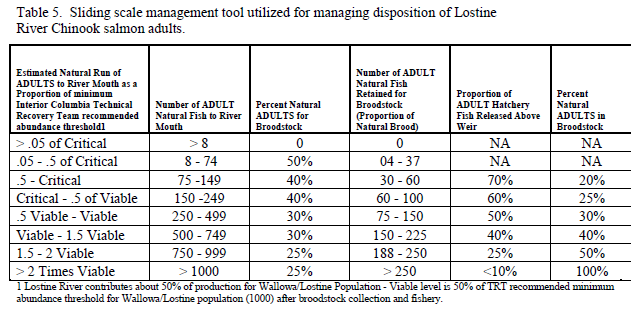
\includegraphics[width=1\linewidth]{./lostine_sliding_scale} 

}

\caption{Copied from the 2011 Hatchery and Genetic Management Plan for Grande Ronde Spring Chinook Salmon Supplementation Program.}\label{fig:lostine-sliding-scale}
\end{figure}

\subsection{Limitations of the Existing Framework}\label{limitations-of-the-existing-framework}

The sliding scale has successfully guided Lostine River weir management for more than a decade and has provided a transparent and repeatable process for balancing conservation and production objectives. Nevertheless, several characteristics of the framework create operational complexities, limit managers' ability to achieve program objectives, and constrain the incorporation of new biological information into management decisions.

First, operational complexities arise when natural- and hatchery-origin abundance forecasts are updated in season. As forecasts change, they may cross predefined abundance thresholds, causing abrupt shifts in broodstock composition and hatchery fish disposition. Consequently, relatively small differences in estimated abundance can result in substantially different management actions despite little biological difference between return sizes.

Second, integrated supplementation programs are intended to increase natural production and provide harvest opportunities by allowing hatchery-origin fish to contribute to natural spawning while maintaining acceptable levels of genetic risk. Under the current sliding scale, high natural-origin returns can trigger increased removal of hatchery-origin fish at the weir, thereby reducing the number of hatchery fish available to spawn naturally. This can limit the demographic contribution of the hatchery program and reduce future production and harvest opportunities, even when natural-origin abundance is sufficient to meet broodstock and spawning objectives.

Third, the abundance thresholds and associated assumptions regarding genetic risk were developed more than 15 years ago using the best information available at that time. Since implementation of the HGMP, extensive monitoring has substantially improved our understanding of supplementation outcomes in the Lostine River and other spring/summer Chinook Salmon populations \autocite{hess_supportive_2012,janowitzkoch_long-term_2019}. These data include long-term records of adult abundance, juvenile production, broodstock performance, natural spawning, spawner-recruit relationships, and genetic parentage analyses that directly evaluate the reproductive success of hatchery- and natural-origin fish. The current sliding-scale framework has limited flexibility to incorporate this growing body of scientific information without revising the threshold structure itself.

Finally, because the sliding scale is based on fixed abundance categories, adapting the framework requires modifying decision thresholds rather than simply updating the biological information that informs management decisions. This makes the framework less responsive to new scientific understanding and more difficult to refine as additional monitoring data become available.

These limitations motivated development of the proposed Anchor Method, which retains the existing harvest framework and management objectives while replacing the stepped broodstock accounting with a continuous, biologically informed relationship between natural-origin abundance and broodstock composition.

\section{Objective 1: Anchor Method Summary}\label{sec:obj1}

The proposed Anchor Method was developed to retain the existing biological objectives, harvest framework, and co-manager decision process while replacing the stepped broodstock accounting of the sliding scale with a continuous, biologically informed relationship. Rather than applying the same management response across broad abundance categories, the Anchor Method adjusts the desired natural-origin contribution to broodstock proportionally based on the estimated natural-origin return and identified spawner goal.

The approach is intended to reduce abrupt changes in management actions near sliding-scale thresholds, make greater use of long-term monitoring information, and provide an accounting framework that can be updated as biological understanding improves. The structure of the method remains fixed, but key biological and operational inputs---including the spawner goal, broodstock need, fishery impacts, trap proportions, weir efficiency, and pre-spawn survival---can be revised through the co-manager process.

\subsection{Conceptual Overview}\label{conceptual-overview}

The Anchor Method does not propose a new harvest policy or a new set of biological objectives. Rather, it proposes a different accounting framework for allocating adults after natural-origin (NOR) and hatchery-origin (HOR) abundance have been estimated. The existing FMEP harvest relationships, treaty and non-treaty allocation framework, annual broodstock need, and overall objectives of the integrated hatchery program remain unchanged.

The largest change in the new approach is a replacement of the stepped broodstock targets of the sliding scale with a continuous relationship between NOR abundance and the desired proportion of natural-origin broodstock. This relationship is established using a calculated benchmark referred to as the \textbf{Anchor}.

The Anchor is separate from the annual mixed-origin accounting. It is not an escapement target, a run-size forecast, or a desired number of fish to manage toward in a particular year. Instead, it is a reference abundance used to determine the natural-origin contribution to broodstock under a given management scenario.

\subsection{The Anchor}\label{the-anchor}

The Anchor represents the minimum NOR adult abundance required to satisfy two conditions under the assumption that the entire broodstock is composed of natural-origin fish:

\begin{enumerate}
\def\labelenumi{\arabic{enumi}.}
\tightlist
\item
  enough NOR adults remain after expected fishery impacts to fill the full broodstock need; and
\item
  enough NOR adults survive to spawning to achieve the adult spawner goal.
\end{enumerate}

The Anchor is determined by evaluating a sequence of candidate NOR abundances. For each candidate abundance, the accounting applies projected NOR fishery impacts, partitions the remaining adults at the weir, allocates broodstock entirely from captured NOR fish, applies pre-spawn survival, and evaluates whether both the broodstock requirement and spawner goal are met. The smallest candidate abundance satisfying both conditions and becomes the Anchor.

The Anchor therefore depends on several assumptions and inputs, including:

\begin{itemize}
\tightlist
\item
  annual broodstock need;
\item
  adult spawner goal;
\item
  FMEP fishery impact relationships;
\item
  the Wallowa/Lostine population scaling factor;
\item
  the proportion of NOR adults captured at the weir;
\item
  weir efficiency; and
\item
  pre-spawn survival above and below the weir.
\end{itemize}

Once the Anchor is calculated, the desired annual proportion of natural-origin broodstock is determined from the ratio of the NOR forecasted abundance to the Anchor:

\[
\text{desired pNOB} =
\min\left(1,\frac{\text{NOR abundance}}{\text{Anchor}}\right).
\]

When NOR abundance equals or exceeds the Anchor, the desired pNOB is 1.0. When NOR abundance is below the Anchor, the desired pNOB declines proportionally. For example, an estimated NOR abundance equal to one-half of the Anchor produces a desired pNOB of 0.5.

\subsection{Management Priorities}\label{management-priorities}

The Anchor Method follows a sequential accounting process based on our review of the current functions and supporting documentation. The practical priorities of the method are:

\begin{enumerate}
\def\labelenumi{\arabic{enumi}.}
\tightlist
\item
  Establish an agreed upon spawner goal from available information.
\item
  Calculate a desired natural-origin broodstock contribution (pNOB) from the Anchor relationship.
\item
  Protect the availability of enough NOR and HOR adults to satisfy the broodstock requirement.
\item
  Apply fisheries to the extent allowed using the existing harvest impact relationships and origin specific broodstock requirements.
\item
  Allocate captured adults to broodstock.
\item
  Estimate the number of NOR and HOR adults expected to survive to spawn naturally.
\item
  Pass all remaining NOR fish and the balance of captured HOR adults upstream to achieve the adult spawner goal.
\item
  Remove remaining excess of captured HOR adults after broodstock allocation and necessary upstream passage.
\end{enumerate}

This sequence contains an important distinction. Fisheries are reduced when projected impacts or harvest would leave too few adults available to meet the broodstock target. However, the current accounting does \textbf{not} further reduce fisheries specifically to reserve fish for the spawner goal. Instead, after fisheries and broodstock collection have occurred, captured HOR fish are passed upstream when additional spawners are needed to meet the desired goal.

Consequently, broodstock receives explicit protection from fisheries, whereas the spawner goal is addressed later through the disposition of available HOR adults. If insufficient NOR and HOR adults remain after fisheries and broodstock collection, the calculated spawner goal may not be achieved. Conversely, once the spawner goal is met, additional HOR fish will be removed and not allowed to spawned.

\subsection{Accounting Sequence}\label{accounting-sequence}

\subsubsection{Fishery calculations and broodstock protection}\label{fishery-calculations-and-broodstock-protection}

For a given management scenario, preliminary NOR fishery impacts are first calculated using the existing sport and treaty harvest relationships. Preliminary HOR harvest is then estimated using the existing fishery allocation and catch-balancing assumptions.

The method evaluates whether the projected fisheries would leave enough adults to meet broodstock needs. The desired number of NOR broodstock is calculated from the Anchor-based pNOB relationship. The number of NOR adults that must remain after fisheries is then estimated from the expected proportion captured at the weir.

If projected NOR impacts would leave too few NOR adults to meet the desired NOR broodstock contribution, sport and treaty NOR impacts are reduced proportionally. A similar cap is applied to HOR harvest when HOR adults are needed to fill the portion of broodstock demand not expected to be met by NOR fish.

These caps protect broodstock availability while retaining the relative allocation of impacts or harvest between fisheries. They do not independently reserve fish for natural spawning.

\subsubsection{Post-fishery weir partitioning}\label{post-fishery-weir-partitioning}

Following fisheries, the remaining NOR and HOR adults are partitioned into three groups:

\begin{enumerate}
\def\labelenumi{\arabic{enumi}.}
\tightlist
\item
  adults captured at the weir;
\item
  adults that pass above the weir without being captured; and
\item
  adults remaining below the weir.
\end{enumerate}

The number captured is determined using origin-specific trap proportions. Weir efficiency is then used to estimate the number of adults that passed above the structure without being captured. Remaining adults are assigned below the weir.

This accounting distinguishes the proportion of the total return captured at the weir from weir efficiency. The trap proportion describes how many adults from the management-area return were captured, including fish that may never have reached the weir. Weir efficiency describes the probability of capture among fish that encountered or passed the weir and is used to estimate uncaptured passage above it.

\subsubsection{Broodstock allocation}\label{broodstock-allocation}

Captured NOR adults are allocated to broodstock first, up to the desired NOR contribution determined by the Anchor relationship. Captured HOR adults are then used to fill any remaining broodstock need.

The resulting realized pNOB may differ from the desired pNOB when too few NOR adults are captured at the weir. Final pNOB is therefore calculated from the realized broodstock allocation rather than directly from the Anchor slope:

\[
\text{pNOB} =
\frac{\text{NOR broodstock}}{\text{total broodstock need}}.
\]

\subsubsection{Natural spawner accounting}\label{natural-spawner-accounting}

After broodstock allocation, remaining adults are evaluated as potential natural spawners. NOR adults captured but not used for broodstock are treated as available for passage above the weir. NOR and HOR adults that passed the weir without capture, as well as adults remaining below the weir, also contribute to the estimated spawning population.

Pre-spawn survival is applied separately to fish above and below the weir. Adults are not counted as spawners merely because they were present in the river or passed above the weir; they contribute to the final spawner estimate only after the applicable survival rate has been applied.

\subsubsection{HOR passage and removal}\label{hor-passage-and-removal}

The accounting next compares the estimated number of spawners with the adult spawner goal. If the estimated spawning population is below the goal, captured HOR adults remaining after broodstock collection are passed above the weir, up to the number expected to close the deficit after accounting for pre-spawn survival.

Captured HOR adults are therefore passed upstream only when needed to achieve the spawner goal. Once the goal has been achieved, or when all available HOR adults have been used, any remaining captured HOR adults are removed from the system.

This decision rule produces predictable outcomes across return conditions. At low NOR abundance, more HOR adults may be required for broodstock and natural spawning, generally resulting in higher pHOS. At high NOR abundance, fewer HOR adults are needed to achieve either objective, generally resulting in greater HOR removal and pHOS approaching zero.

\subsection{Comparison with the Sliding Scale}\label{comparison-with-the-sliding-scale}

The Anchor Method retains much of the existing management framework but changes how desired broodstock composition is determined. The principal differences are summarized in Table \ref{tab:framework-comparison}.

\begin{longtable}[t]{>{\raggedright\arraybackslash}p{2.0in}>{\raggedright\arraybackslash}p{2.0in}>{\raggedright\arraybackslash}p{2.0in}}
\caption{\label{tab:framework-comparison}Conceptual comparison of the existing sliding-scale framework and the proposed Anchor Method.}\\
\toprule
Characteristic & Existing Sliding Scale & Proposed Anchor Method\\
\midrule
\endfirsthead
\caption[]{\label{tab:framework-comparison}Conceptual comparison of the existing sliding-scale framework and the proposed Anchor Method. \textit{(continued)}}\\
\toprule
Characteristic & Existing Sliding Scale & Proposed Anchor Method\\
\midrule
\endhead

\endfoot
\bottomrule
\endlastfoot
Broodstock decision structure & Discrete abundance categories & Continuous relationship with NOR abundance\\
Basis for desired pNOB & Predetermined values within each abundance category & NOR abundance relative to the calculated Anchor\\
Transition between management responses & Abrupt change when a threshold is crossed & Gradual change as NOR abundance changes\\
Harvest framework & Existing FMEP relationships & Existing FMEP relationships retained\\
Harvest constraint & Broodstock and program requirements & Explicit origin-specific broodstock-protection caps\\
\addlinespace
Spawner management & HOR passage determined from sliding-scale prescriptions & HOR passed when needed to support the spawner goal\\
pHOS & Outcome of weir management & Outcome of spawner accounting and HOR passage\\
PNI & Outcome of pNOB and pHOS & Outcome of pNOB and pHOS\\
Ability to incorporate new information & Requires modification of categories or prescribed values & Biological and operational inputs can be updated without changing the basic structure\\*
\end{longtable}

\subsection{Management Defined Spawner Goals}\label{management-defined-spawner-goals}

The predefined spawner goal drives the number of NOR fish that will be retained for broodstock and the point HOR fish will be removed from natural spawning. The proportion of NOR broodstock is calculated as the forecasted NOR return divided by the anchor, with the anchor being derived from the spawner goal. Figure \ref{fig:calc-anchor-range} illustrates the linear dependency between the two values. Thus, using the anchor method managers can easily alter the number of NOR fish being retained for broodstock and the number of HOR fish removed by setting lower or higher spawner goals. Which, will also indirectly influence harvest impacts.

Given the importance of the set spawner goal in the anchor method calculations, managers will need to establish this threshold carefully. Figures \ref{fig:odfw-prod-curves} and \ref{fig:stock-recruit} illustrate the potential differences that may occur when establishing the spawner goal. ODFW initially proposed a spawner goal of 800 based on the Beverton-Holt stock-recruit relationship shown in panel three of Figure \ref{fig:odfw-prod-curves}. While a slightly different Lostine River dataset (provided by B. Simmons) and a Ricker stock-recruit model might suggest a much higher spawner goal (Figure \ref{fig:stock-recruit}). These two approaches could lead to a \textgreater50\% difference in pNOB and the allowable number of HOR fish released upstream.

\begin{figure}[H]

{\centering 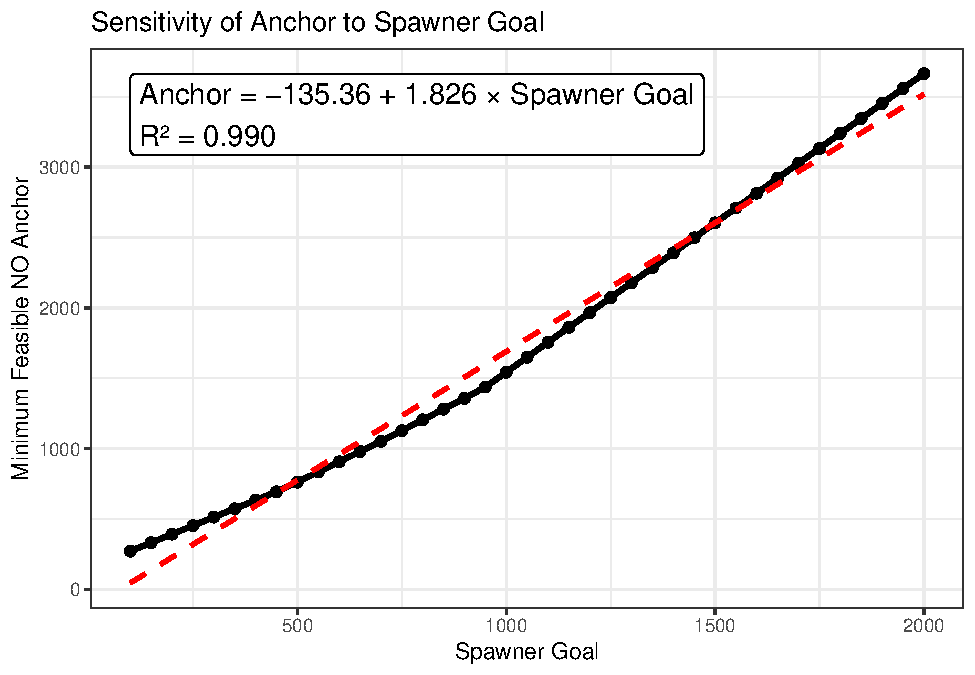
\includegraphics[width=1\linewidth]{anchor_method_evaluation_files/figure-latex/calc-anchor-range-1} 

}

\caption{A linear relationship exists between the calculated anchor and the management set spawner goal.}\label{fig:calc-anchor-range}
\end{figure}

\begin{figure}[H]

{\centering 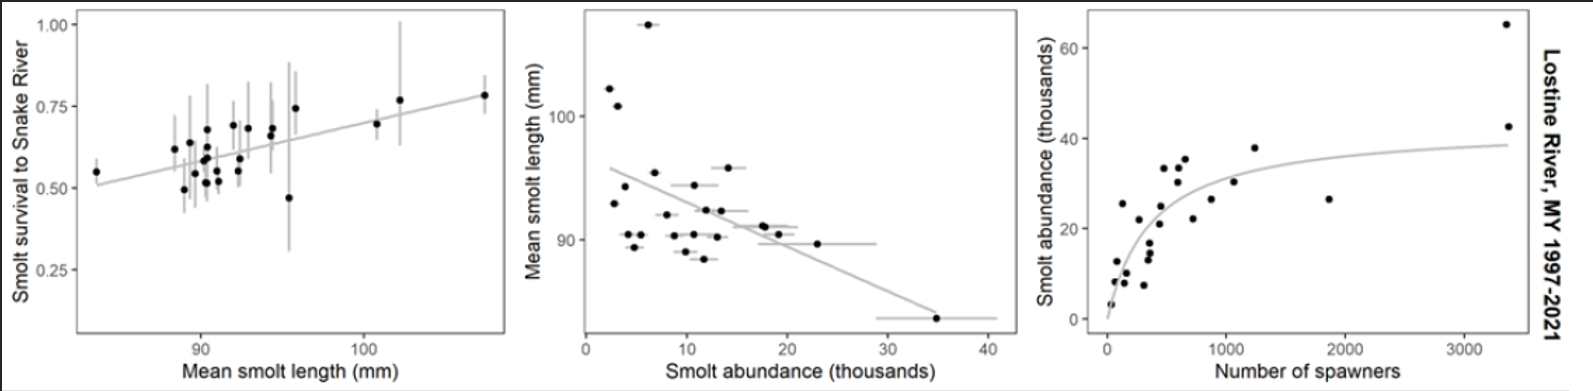
\includegraphics[width=1\linewidth]{./odfw_prod_curves} 

}

\caption{Oregon Department of Fish and Wildlife estimated productivity curves used to set a spawner goal of 800.}\label{fig:odfw-prod-curves}
\end{figure}

\begin{figure}[H]

{\centering \includegraphics[width=1\linewidth]{../../../Chinook-Life-Cycle/figures/plot-smolt-1} 

}

\caption{Beverton-Holt and Ricker stock-recruit curves fit to smolt and spawner abundance in the Lostine River. Data provided by Brian Simmons and it includes brood years 1995-2018.}\label{fig:stock-recruit}
\end{figure}

\subsection{Summary}\label{summary}

The Anchor Method replaces the discrete broodstock prescriptions of the sliding scale with a continuous relationship between NOR abundance and desired pNOB. Its accounting sequence explicitly protects broodstock availability, applies the existing fishery framework, estimates spawners after pre-spawn survival, passes captured HOR adults when needed to support the spawner goal, and removes remaining captured HOR adults.

The approach provides a transparent connection between assumed biological conditions and resulting management actions. However, the method does not explicitly optimize harvest, constrain pHOS or PNI to management thresholds, or guarantee achievement of the spawner goal under all return conditions. Those quantities remain outcomes of the sequential accounting process.

Although the conceptual differences between the sliding scale and Anchor Method are clear their practical importance depends on whether they produce meaningfully different management outcomes under observed return conditions. Objective 2 therefore evaluates how application of the Anchor Method would have changed broodstock composition, harvest, natural spawning, and HOR disposition during recent management years.

\section{Objective 2: Anchor Method Comparison to Sliding Scale (Lostine River)}\label{sec:obj2}

To evaluate the proposed Anchor Method, we compared the predicted total number of natural spawning adults under the Anchor Method with the realized total number of spawners estimated in the Lostine River under the existing sliding-scale framework. For annual calculations, the Anchor Method was parameterized using the ODFW proposed adult spawner goal of 800 fish, a Wallowa--Lostine scaling factor of 1.4, and a broodstock requirement of 160 fish. In addition to the predicted number of spawners, we estimated the number of hatchery-origin fish that would have been removed at the weir under the Anchor Method. Comparisons of other performance metrics, such as hatchery-origin removals, broodstock and spawner composition, pHOS, pNOB, and PNI, were not possible because corresponding realized estimates were not available.

Figure \ref{fig:annual-comparison} compares the predicted total number of spawners under the Anchor Method with the realized number of spawners observed under the sliding-scale framework. In several years, the observed number of spawners exceeded the number predicted by the Anchor Method. These differences were primarily associated with years in which the Lostine River weir experienced operational challenges or reduced trapping efficiency, allowing additional fish to pass upstream regardless of the management framework. In years when the weir operated as intended, the Anchor Method generally resulted in slightly more total spawners than were observed under the sliding-scale approach. However, these differences were typically small and are unlikely to produce biologically meaningful changes in natural production or substantially alter the potential genetic effects associated with hatchery-origin fish spawning naturally.

The stacked bars in Figure \ref{fig:annual-comparison} partition the Anchor Method outcomes into the predicted number of natural spawners and the number of hatchery-origin fish removed at the weir. Together, these values represent the total number of fish available after fisheries and illustrate how fish are allocated between natural spawning and removal once broodstock and adult spawner objectives have been achieved. In 2008, 2009, 2012, 2015, 2016, 2018, and 2022, the predicted number of natural spawners under the Anchor Method reached the 800-fish spawner goal. Although additional hatchery-origin fish were available in those years, they would have been removed because the management objectives had already been satisfied and additional spawners were not required.

\begin{figure}[H]

{\centering 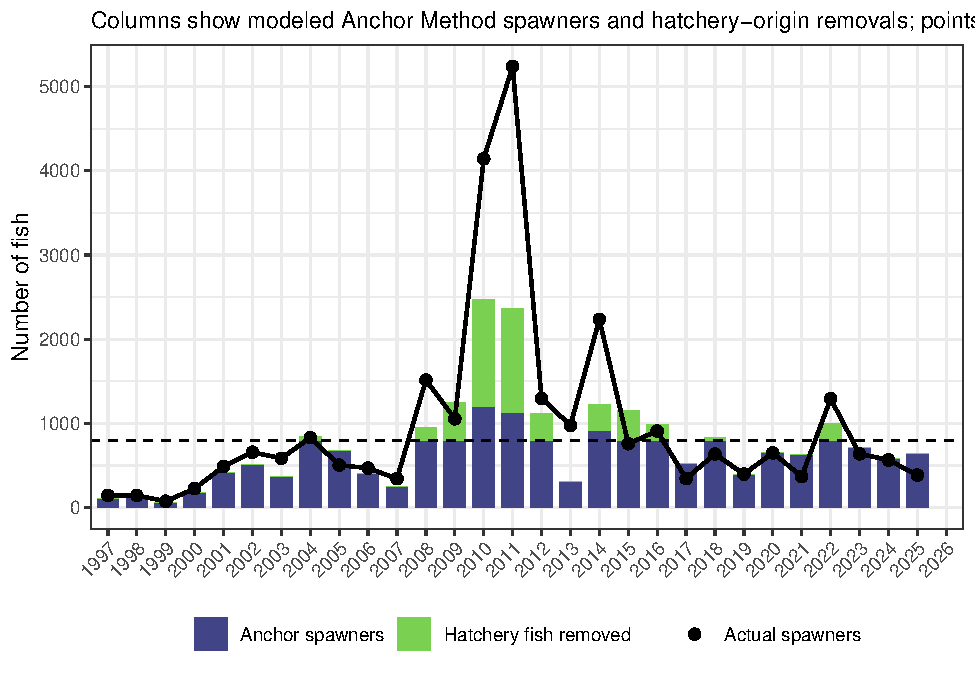
\includegraphics[width=1\linewidth]{anchor_method_evaluation_files/figure-latex/annual-comparison-1} 

}

\caption{Predicted anchor method total spawners and hatchery removals versus the actual number of total spawners.}\label{fig:annual-comparison}
\end{figure}

\section{Objective 3: Sensitivity of the Anchor Method}\label{sec:obj3}

The sensitivity analysis evaluated how modeled management outcomes changed across combinations of natural-origin abundance, hatchery-origin abundance, and adult spawner goals ranging from 400 to 1,400 fish. The results are organized around the three primary components of the accounting framework: treaty harvest, natural spawning, and broodstock composition.

\subsection{Treaty Harvest}\label{treaty-harvest}

Treaty harvest was most constrained when natural-origin abundance was low relative to broodstock and spawning requirements. The harvest boundary (Figure \ref{fig:treaty-harvest-decision} identifies combinations of NOR and HOR abundance for which modeled treaty impacts on NOR fish were limited to fewer than 50 fish. The corresponding response surface (Figure \ref{fig:treaty-harvest}) shows that treaty impacts generally increased with natural-origin abundance, but the abundance at which additional impacts became available was not depended on the spawner goal. This result is expected and follows the identified prioritization of fish allocation within the anchor method (Section \ref{sec:obj1}). Treaty impacts on NOR fish only increased linearly with NOR abundance as expected and was not dependent on HOR abundance or the spawner goal (Figure \ref{fig:nor-treaty-impacts})

\subsection{Natural Spawning}\label{natural-spawning}

The modeled number of total spawners increased with both NOR and HOR abundance until the applicable spawner goal was reached (Figure \ref{fig:total-spawners-sensitivity}). Once the goal was achieved, additional hatchery-origin fish were generally removed rather than passed upstream (Figure \ref{fig:hor-removals-decision}). The hatchery-removal decision boundary therefore shifted with the spawner goal: higher goals required more fish to remain available for natural spawning before removals began. The removal response surface further illustrates that the number of hatchery-origin fish removed was greatest when hatchery-origin abundance was high and the spawner goal could be achieved without passing all available fish (Figure \ref{fig:hor-removals}). The resulting pHOS values reflected the relative availability of NOR and HOR fish and the number of HOR fish retained for natural spawning (Figure \ref{fig:phos-sensitivity}).

\subsection{Broodstock Composition}\label{broodstock-composition}

Broodstock composition also varied predictably across abundance scenarios (Figure \ref{fig:pnob-sensitivity}). The pNOB target increased linearly with NOR abundance because a greater proportion of the broodstock requirement could be met with natural-origin fish. As the spawner goal increased pNOB decreased because the NOR abundance became a smaller proportion of the set anchor. PNI followed the combined response of pNOB and pHOS and was highest in scenarios with high natural-origin representation in broodstock and relatively low hatchery-origin representation among natural spawners (Figure \ref{fig:pni-sensitivity}).

\subsection{Conclusion}\label{conclusion}

Collectively, these results demonstrate that the Anchor Method responds continuously to changes in annual return composition while maintaining the established sequence of management priorities. Broodstock and natural-spawning requirements constrain harvest when natural-origin abundance is low, whereas hatchery removals become more likely after broodstock and spawner objectives have been achieved. Increasing the spawner goal shifts management decisions to fewer HOR removals and a lower pNOB and PNI.

\begin{figure}[H]

{\centering 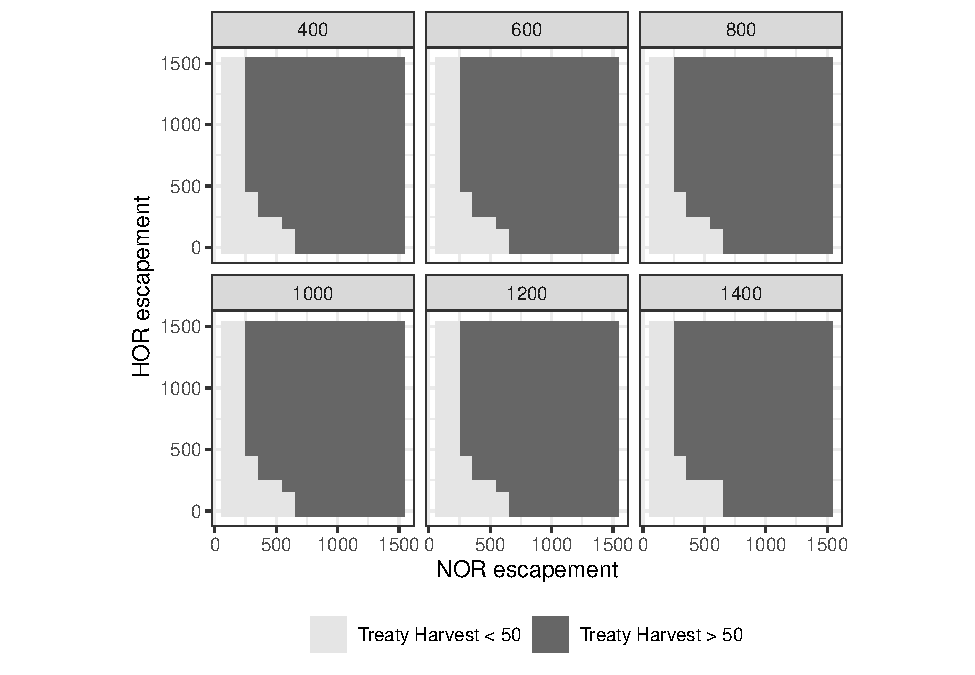
\includegraphics[width=1\linewidth]{anchor_method_evaluation_files/figure-latex/treaty-harvest-decision-1} 

}

\caption{Estimated treaty harvest less than 50 fish (NOR + HOR) using the "Anchor Method" at varying levels of natural-origin (NOR) and hatchery-origin (HOR) escapment on the x- and y-axis, and at different management spawner goals for each facet. The light grey depicts abundances where harvest is less than 50.}\label{fig:treaty-harvest-decision}
\end{figure}

\begin{figure}[H]

{\centering 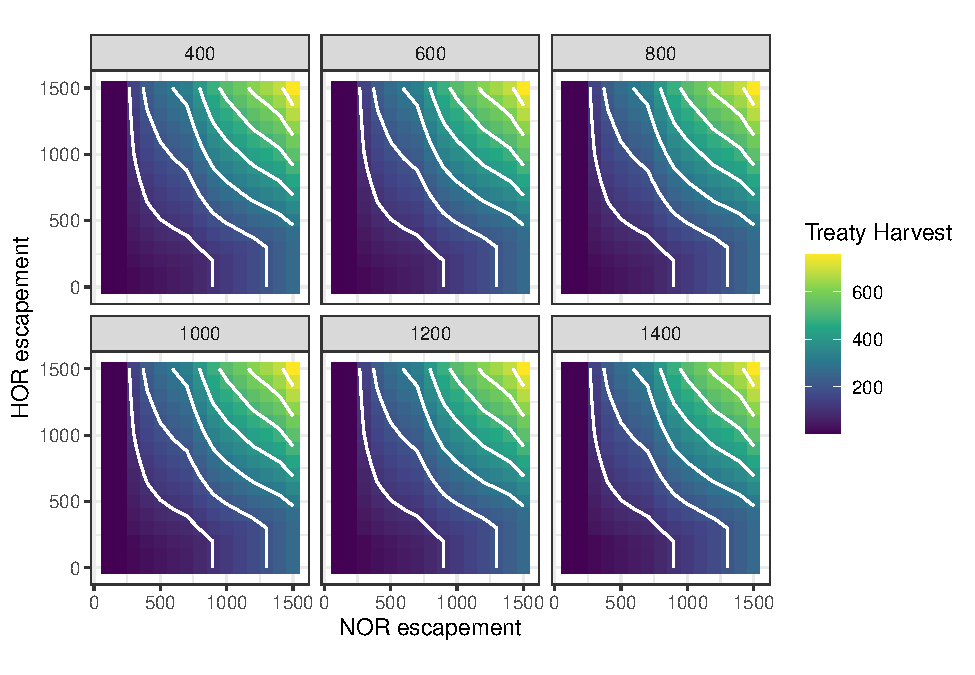
\includegraphics[width=1\linewidth]{anchor_method_evaluation_files/figure-latex/treaty-harvest-1} 

}

\caption{Predicted total treaty harvest (NOR + HOR) using the "Anchor Method" at varying levels of natural-origin (NOR) and hatchery-origin (HOR) escapment on the x- and y-axis, and at different management spawner goals for each facet.}\label{fig:treaty-harvest}
\end{figure}

\begin{figure}[H]

{\centering 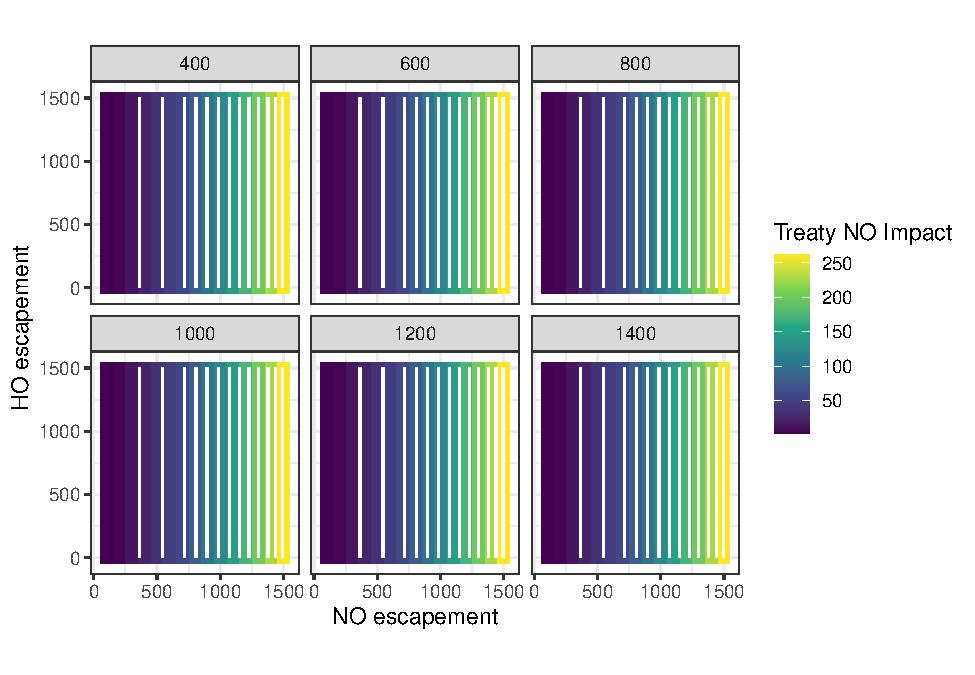
\includegraphics[width=1\linewidth]{anchor_method_evaluation_files/figure-latex/nor-treaty-impacts-1} 

}

\caption{Predicted natural-origin treaty impact rate harvest using the "Anchor Method" at varying levels of natural-origin (NOR) and hatchery-origin (HOR) escapment on the x- and y-axis, and at different management spawner goals for each facet.}\label{fig:nor-treaty-impacts}
\end{figure}

\begin{figure}[H]

{\centering 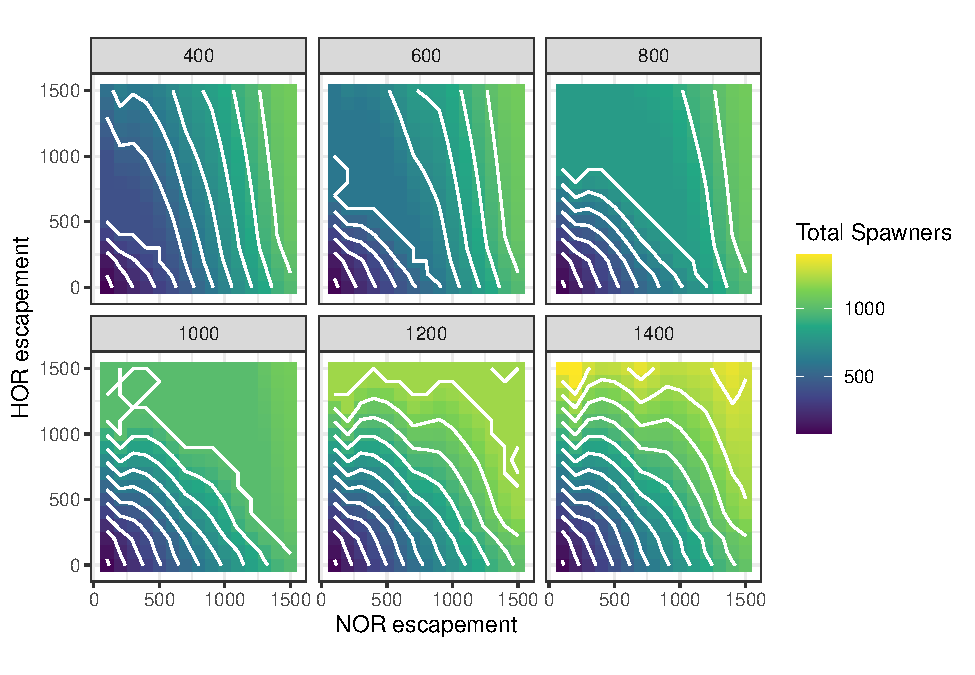
\includegraphics[width=1\linewidth]{anchor_method_evaluation_files/figure-latex/total-spawners-sensitivity-1} 

}

\caption{Total estimated spawners using the "Anchor Method" at varying levels of natural-origin (NOR) and hatchery-origin (HOR) escapment on the x- and y-axis, and at different management spawner goals for each facet.}\label{fig:total-spawners-sensitivity}
\end{figure}

\begin{figure}[H]

{\centering 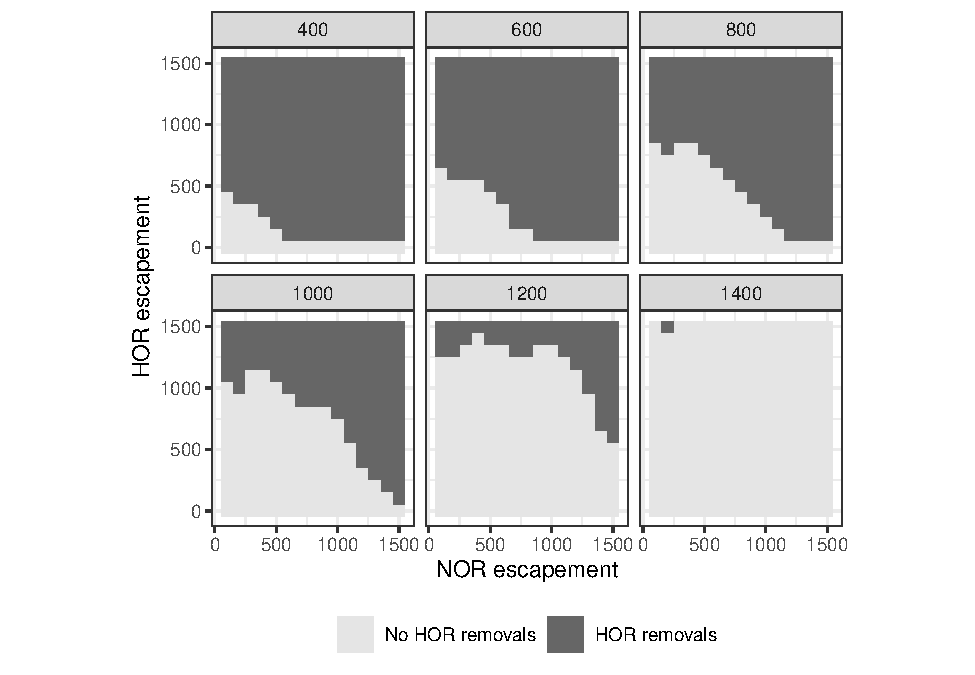
\includegraphics[width=1\linewidth]{anchor_method_evaluation_files/figure-latex/hor-removals-decision-1} 

}

\caption{Hatchery-origin removal decisions points using the "Anchor Method" at varying levels of natural-origin (NOR) and hatchery-origin (HOR) escapment on the x- and y-axis, and at different management spawner goals for each facet. The light grey depicts abundances allowing all HOR fish to be utilized for broodstock, harvest, or spawning, the dark grey indicates abundances when some HOR fish would be removed.}\label{fig:hor-removals-decision}
\end{figure}

\begin{figure}[H]

{\centering 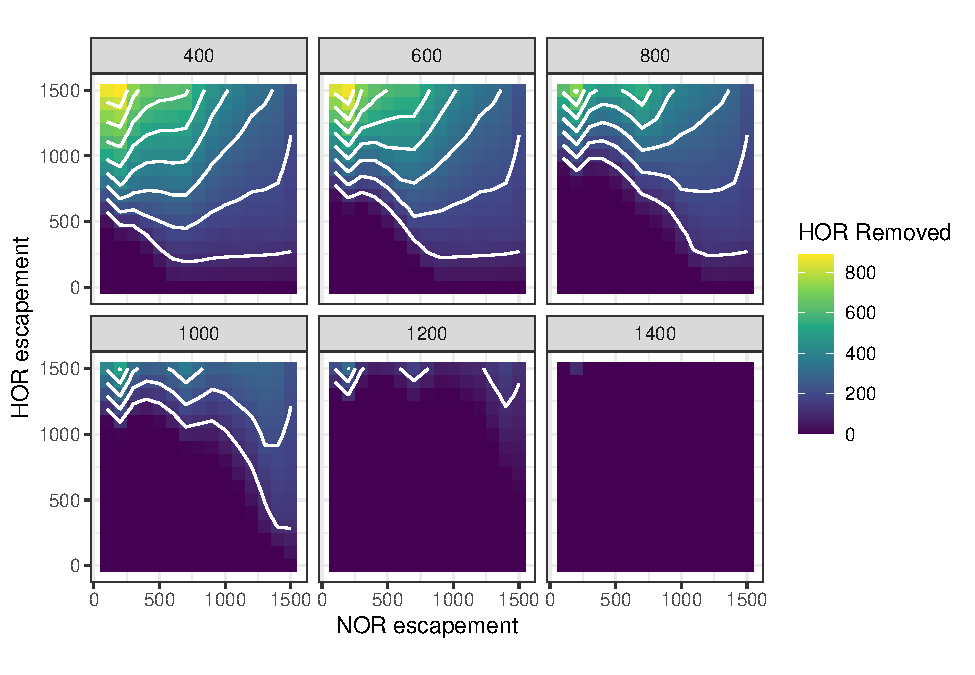
\includegraphics[width=1\linewidth]{anchor_method_evaluation_files/figure-latex/hor-removals-1} 

}

\caption{Predicted number of hatchery-origin removals using the "Anchor Method" at varying levels of natural-origin (NOR) and hatchery-origin (HOR) escapment on the x- and y-axis, and at different management spawner goals for each facet.}\label{fig:hor-removals}
\end{figure}

\begin{figure}[H]

{\centering 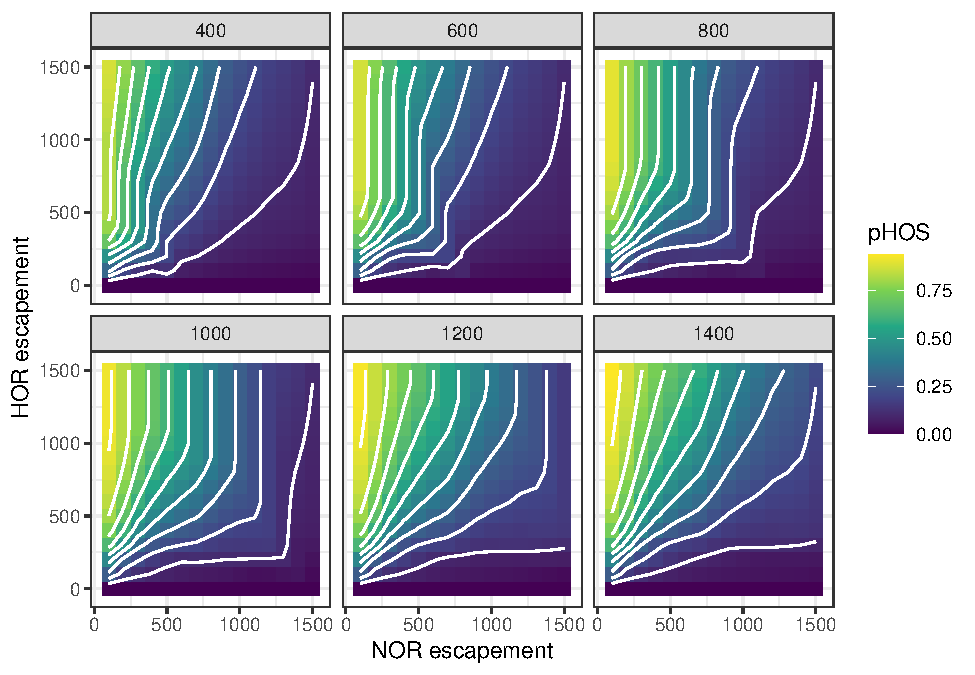
\includegraphics[width=1\linewidth]{anchor_method_evaluation_files/figure-latex/phos-sensitivity-1} 

}

\caption{Calculated proportion of hatchery-origin spawners (pHOS) using the "Anchor Method" at varying levels of natural-origin (NOR) and hatchery-origin (HOR) escapment on the x- and y-axis, and at different management spawner goals for each facet.}\label{fig:phos-sensitivity}
\end{figure}

\begin{figure}[H]

{\centering 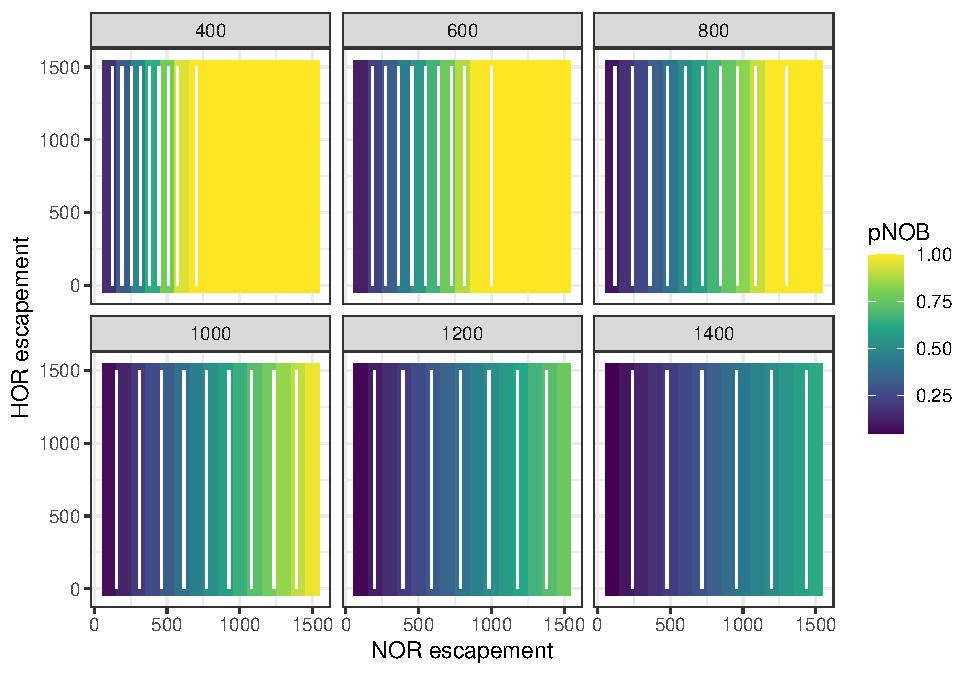
\includegraphics[width=1\linewidth]{anchor_method_evaluation_files/figure-latex/pnob-sensitivity-1} 

}

\caption{Proposed proportion of natural-origin broodstock (pNOB) target using the "Anchor Method", at varying levels of natural-origin (NOR) and hatchery-origin (HOR) escapment on the x- and y-axis, and at different management spawner goals for each facet.}\label{fig:pnob-sensitivity}
\end{figure}

\begin{figure}[H]

{\centering 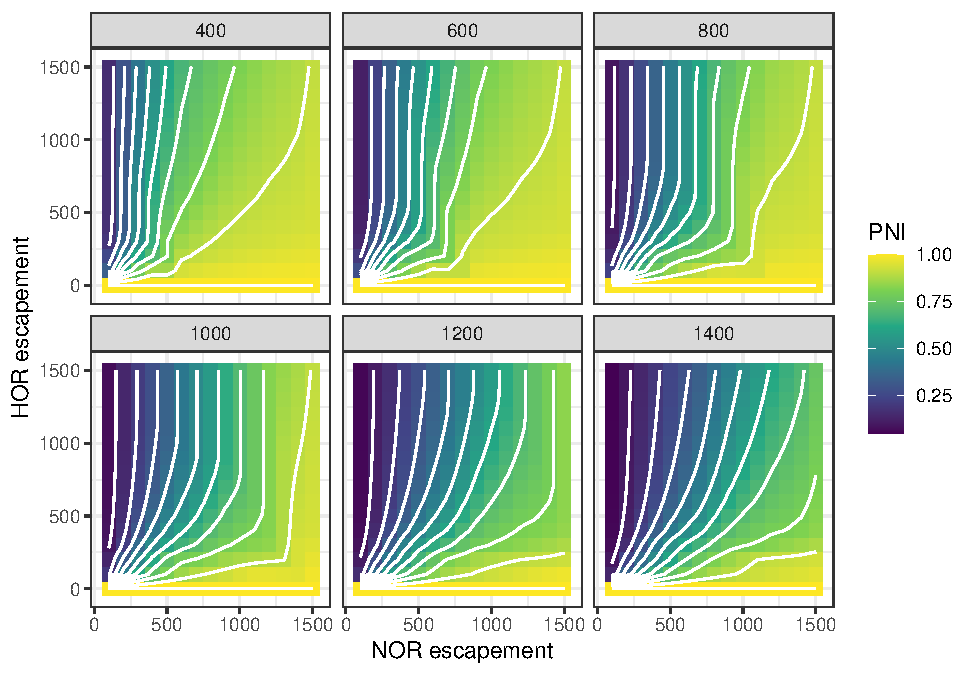
\includegraphics[width=1\linewidth]{anchor_method_evaluation_files/figure-latex/pni-sensitivity-1} 

}

\caption{Proposed proportion of natural influence using the "Anchor Method", at varying levels of natural-origin (NOR) and hatchery-origin (HOR) escapment on the x- and y-axis, and at different management spawner goals for each facet.}\label{fig:pni-sensitivity}
\end{figure}

% References (only if bibliography present)
\section*{References}
\printbibliography[heading=none]


\end{document}
